%-*-latex-*-
\sectionthree{Sentinel node}
\begin{python0}
from solutions import *; clear()
\end{python0}

A \defone{sentinel node} is a dummy node.
It does not hold data.
Let me show you what I mean.
Look at this singly linked list:

\begin{center}
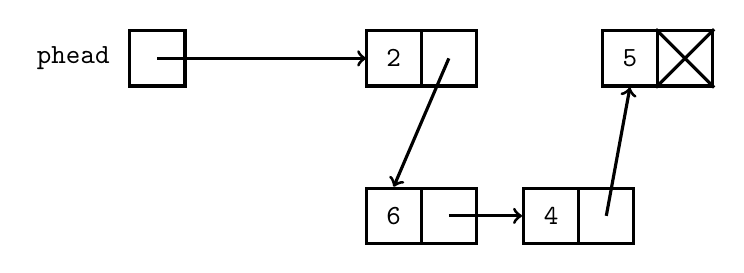
\begin{tikzpicture}

\draw (0.35, 0.35)
  node[draw, line width=0.04cm, , color=black,
       rounded corners=0cm, inner sep=0cm] {

\begin{minipage}[t][0.7cm]{0.7cm}
\mbox{}

\end{minipage}

};\draw (0.35, 0.35) node[color=black] {{\texttt{2}}};
\draw (1.0499999999999998, 0.35)
  node[draw, line width=0.04cm, , color=black,
       rounded corners=0cm, inner sep=0cm] {

\begin{minipage}[t][0.7cm]{0.7cm}
\mbox{}

\end{minipage}

};\draw (1.0499999999999998, 0.35) node[color=black] {{\texttt{}}};
\draw (0.35, -1.65)
  node[draw, line width=0.04cm, , color=black,
       rounded corners=0cm, inner sep=0cm] {

\begin{minipage}[t][0.7cm]{0.7cm}
\mbox{}

\end{minipage}

};\draw (0.35, -1.65) node[color=black] {{\texttt{6}}};
\draw (1.0499999999999998, -1.65)
  node[draw, line width=0.04cm, , color=black,
       rounded corners=0cm, inner sep=0cm] {

\begin{minipage}[t][0.7cm]{0.7cm}
\mbox{}

\end{minipage}

};\draw (1.0499999999999998, -1.65) node[color=black] {{\texttt{}}};
\draw (2.35, -1.65)
  node[draw, line width=0.04cm, , color=black,
       rounded corners=0cm, inner sep=0cm] {

\begin{minipage}[t][0.7cm]{0.7cm}
\mbox{}

\end{minipage}

};\draw (2.35, -1.65) node[color=black] {{\texttt{4}}};
\draw (3.0500000000000003, -1.65)
  node[draw, line width=0.04cm, , color=black,
       rounded corners=0cm, inner sep=0cm] {

\begin{minipage}[t][0.7cm]{0.7cm}
\mbox{}

\end{minipage}

};\draw (3.0500000000000003, -1.65) node[color=black] {{\texttt{}}};
\draw (3.35, 0.35)
  node[draw, line width=0.04cm, , color=black,
       rounded corners=0cm, inner sep=0cm] {

\begin{minipage}[t][0.7cm]{0.7cm}
\mbox{}

\end{minipage}

};\draw (3.35, 0.35) node[color=black] {{\texttt{5}}};
\draw (4.05, 0.35)
  node[draw, line width=0.04cm, , color=black,
       rounded corners=0cm, inner sep=0cm] {

\begin{minipage}[t][0.7cm]{0.7cm}
\mbox{}

\end{minipage}

};\draw (4.05, 0.35) node[color=black] {{\texttt{}}};\draw[line width=0.04cm,black,->] (1.05,0.35) to  (0.35,-1.28);
\draw[line width=0.04cm,black,->] (1.05,-1.65) to  (1.98,-1.65);
\draw[line width=0.04cm,black,->] (3.05,-1.65) to  (3.35,-0.02);
\draw[line width=0.04cm,black] (3.68,0.72) to  (4.42,-0.02);
\draw[line width=0.04cm,black] (4.42,0.72) to  (3.68,-0.02);

\draw (-2.65, 0.35)
  node[draw, line width=0.04cm, , color=black,
       rounded corners=0cm, inner sep=0cm] {

\begin{minipage}[t][0.7cm]{0.7cm}
\mbox{}

\end{minipage}

};\draw (-2.65, 0.35) node[color=black] {{\texttt{}}};\draw[line width=0.04cm,black,->] (-2.65,0.35) to  (0,0.35);

\draw (-3.7199999999999998, 0.35)
  node[draw, line width=0.04cm, , color=white,
       rounded corners=0cm, inner sep=0cm] {

\begin{minipage}[t][0.1cm]{0.1cm}
\mbox{}

\end{minipage}

};\draw (-3.7199999999999998, 0.35) node[color=black] {{\texttt{phead}}};
\end{tikzpicture}

\end{center}



Suppose I add a dummy node like this:

\begin{center}
\begin{tikzpicture}
\draw[line width=0.03cm,red,<->] (7) to [bend left=90]  (8);

\fill[blue!10] (0.0, 0.0) circle (0.35);
\node [line width=0.03cm,black,minimum size=0.6699999999999999cm,draw,circle] at (0.0,0.0)(10){};\draw (0.0, 0.0) node[color=black] {\texttt{10}};
\fill[blue!10] (-0.95, -1.0) circle (0.35);
\node [line width=0.03cm,black,minimum size=0.6699999999999999cm,draw,circle] at (-0.95,-1.0)(5){};\draw (-0.95, -1.0) node[color=black] {\texttt{5}};
\fill[blue!10] (0.95, -1.0) circle (0.35);
\node [line width=0.03cm,black,minimum size=0.6699999999999999cm,draw,circle] at (0.95,-1.0)(7){};\draw (0.95, -1.0) node[color=black] {\texttt{7}};
\fill[blue!10] (-1.43, -2.0) circle (0.35);
\node [line width=0.03cm,black,minimum size=0.6699999999999999cm,draw,circle] at (-1.43,-2.0)(2){};\draw (-1.43, -2.0) node[color=black] {\texttt{2}};
\fill[blue!10] (-0.47, -2.0) circle (0.35);
\node [line width=0.03cm,black,minimum size=0.6699999999999999cm,draw,circle] at (-0.47,-2.0)(1){};\draw (-0.47, -2.0) node[color=black] {\texttt{1}};
\fill[blue!10] (0.47, -2.0) circle (0.35);
\node [line width=0.03cm,black,minimum size=0.6699999999999999cm,draw,circle] at (0.47,-2.0)(0){};\draw (0.47, -2.0) node[color=black] {\texttt{0}};
\fill[blue!10] (1.43, -2.0) circle (0.35);
\node [line width=0.03cm,black,minimum size=0.6699999999999999cm,draw,circle] at (1.43,-2.0)(8){};\draw (1.43, -2.0) node[color=black] {\texttt{8}};\draw[line width=0.03cm,black] (10) to  (5);
\draw[line width=0.03cm,black] (10) to  (7);
\draw[line width=0.03cm,black] (5) to  (2);
\draw[line width=0.03cm,black] (5) to  (1);
\draw[line width=0.03cm,black] (7) to  (0);
\draw[line width=0.03cm,black] (7) to  (8);
\end{tikzpicture}

\end{center}



Note that that key value of the sentinel node is not used.
I'm using the next pointer of the sentinel node like the pointer to
the head node.

This dummy node is sometimes called the \defone{head sentinel}.
You can think of the head sentinel node as a fake node.

Sentinel nodes can simplify your code.
In the case of insert head, if you use a \verb!phead! pointer, the
code looks like:
\begin{console}
phead = new Node(key, phead)
\end{console}
which is nice and clean an simple.
For delete head, the code looks like
\begin{console}
if phead is NULL:
    throw an exception
else:
    q = phead->next_
    delete phead
    phead = q
\end{console}
Note that in the case of using pointer to head node,
I cannot execute \verb!phead->next_! if \verb!phead! is \verb!NULL!.
That's why the first version of insert head has an if-else.
You don't have this issue if you use a head sentinel --
the head sentinel node is a node.

Instead of using a head sentinel node,
another implemnetation is to use a pointer to a head sentinel node
where the head sentinel node is in the heap.

You can also attach a tail sentinel to the end of the
singly linked list.
Why is this useful?
The tail sentinel can then be used as an end-of-singly-linked-list node.
This helps in writing code that iterates over a singly-linked list:
\begin{console}
p = pheadsentinel->next_
while p is not ptailsentinel
{
    do something with node (*p)
    p = p->next_
}
\end{console}
